\section*{CHƯƠNG 2: LÝ THUYẾT}
\addcontentsline{toc}{section}{\numberline {} CHƯƠNG 2: LÝ THUYẾT}
\setcounter{section}{2}
\setcounter{subsection}{0}
\subsection{CÔNG NGHỆ LORA}
\subsubsection{Khái niệm}
LoRa là viết tắt của Long Range Radio được nghiên cứu và phát triển bởi Cycleo và sau này được mua lại bởi công ty Semtech năm 2012. Với công nghệ này, chúng ta có thể truyền dữ liệu với khoảng cách lên hàng km mà không cần các mạch khuếch đại công suất; từ đó giúp tiết kiệm năng lượng tiêu thụ khi truyền/nhận dữ liệu. Do đó, LoRa có thể được áp dụng rộng rãi trong các ứng dụng thu thập dữ liệu như sensor network trong đó các sensor node có thể gửi giá trị đo đạc về trung tâm cách xa hàng km và có thể hoạt động với battery trong thời gian dài trước khi cần thay pin.\\
\indent Với tầm xa ,nền tảng không dây công suất thấp là sự lựa chọn công nghệ phổ biến hiện hành để xây dựng mạng iot trên thế giới ứng dụng iot thông minh đã cải thiện theo cách tương tác và giải quết giải quyết một số thách thức lớn nhất mà các thành phố và cộng đồng đang phải đối mặt :biến đổi khí hậu ,kiểm soát ô nhiễm cảnh báo thiên tai và cứu mạng .Kinh doanh cũng được hưởng lợi thông qua cũng như giảm được chi phí
Đây là RF công nghệ không dây được tích hợp vào xe ô tô, đèn đường , sản xuất thiết bị , đồ gia dụng thiết bị đeo được bất cứ điều gì , thực sự . Công nghệ Lora đang làm thế giới ta một hành tinh thông minh\\
\indent Dưới đây là hình ảnh để bạn hiểu rõ nét về tầm xa của Lora:
\begin{figure}[H]
	\centering
	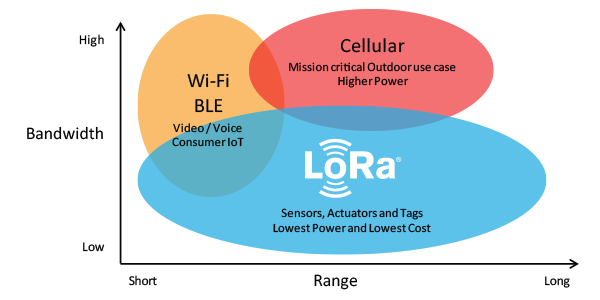
\includegraphics[scale=.5]{Chapter 2/image chapter 2/tamxaLoRa.png}
	\caption[Ảnh minh hoạ tầm xa LoRa]{Ảnh minh hoạ tầm xa LoRa}
	\label{hinh21}
\end{figure}
\subsubsection{Nguyên lý hoạt động}
LoRa sử dụng kỹ thuật điều chế gọi là Chirp Spread Spectrum. Có thể hiểu nôm na nguyên lý này là dữ liệu sẽ được băm bằng các xung cao tần để tạo ra tín hiệu có dãy tần số cao hơn tần số của dữ liệu gốc (cái này gọi là chipped); sau đó tín hiệu cao tần này tiếp tục được mã hoá theo các chuỗi chirp signal (là các tín hiệu hình sin có tần số thay đổi theo thời gian; có 2 loại chirp signal là up-chirp có tần số tăng theo thời gian và down-chirp có tần số giảm theo thời gian; và việc mã hoá theo nguyên tắc bit 1 sẽ sử dụng up-chirp, và bit 0 sẽ sử dụng down-chirp) trước khi truyền ra anten để gửi đi.\\
\indent Theo Semtech công bố thì nguyên lý này giúp giảm độ phức tạp và độ chính xác cần thiết của mạch nhận để có thể giải mã và điều chế lại dữ liệu; hơn nữa LoRa không cần công suất phát lớn mà vẫn có thể truyền xa vì tín hiệu Lora có thể được nhận ở khoảng cách xa ngay cả độ mạnh tín hiệu thấp hơn cả nhiễu môi trường xung quanh.\\
\indent Băng tần làm việc của LoRa từ 430MHz đến 915MHz cho từng khu vực khác nhau trên thế giới:
\begin{itemize}
	\item 430MHz cho châu Á
	\item 780MHz cho Trung Quốc
	\item 433MHz hoặc 866MHz cho châu Âu
	\item 915MHz cho USA
\end{itemize}

\indent Nhờ sử dụng chirp signal mà các tín hiệu LoRa với các chirp rate khác nhau có thể hoạt động trong cùng 1 khu vực mà không gây nhiễu cho nhau. Điều này cho phép nhiều thiết bị LoRa có thể trao đổi dữ liệu trên nhiều kênh đồng thời (mỗi kênh cho 1 chirprate)
\subsubsection{Module thu phát RF UART E32-TTL-100}
\begin{figure}[H]
	\centering
	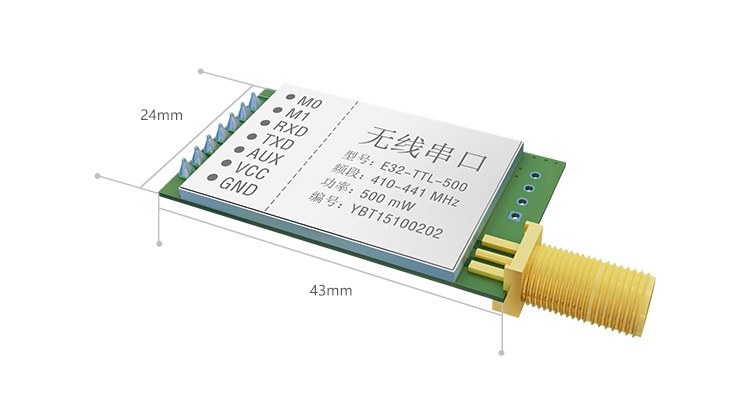
\includegraphics[scale=.4]{Chapter 2/image chapter 2/E32.jpg}
	\caption[Module RF UART E32-TTL-100]{Module RF UART E32-TTL-100}
	\label{hinh22}
\end{figure}
Mạch thu phát RF UART Lora SX1278 433Mhz 3000m sử dụng chip SX1278 của nhà sản xuất SEMTECH chuẩn giao tiếp LORA (Long Range), chuẩn LORA mang đến hai yếu tố quan trọng là tiết kiệm năng lượng và khoảng cách phát siêu xa ( Ultimate long range wireless solution), ngoài ra nó còn có khả năng cấu hình để tạo thành mạng nên hiện tại được phát triển và sử dụng rất nhiều trong các nghiên cứu về IoT.\\
\indent Mạch thu phát RF UART Lora SX1278 433Mhz 3000m được tích hợp phần chuyển đổi giao tiếp SPI của SX1278 sang UART giúp việc giao tiếp và sử dụng rất dễ dàng, chỉ cần kết nối với Software của hãng để cấu hình địa chỉ , tốc độ và công suất truyền là có thể sử dụng.\\
\indent \textbf{Thông số kỹ thuật:}
\begin{itemize}
	\item Model: E32-TTL-100 RF
	\item Điện áp hoạt đông: 2.3 - 5.5 VDC
	\item Điện áp giao tiếp: TTL-3.3V
	\item Giao tiếp UART Data bits 8, Stop bits 1, Parity none, tốc độ từ 1200 - 115200.
	\item Tần số: 410 - 441Mhz
	\item Công suất: 20dbm (100mW)
	\item Khoảng cách truyền tối đa trong điều kiện lý tưởng: 3000m
	\item Tốc độ truyền: 0.3 - 19.2 Kbps ( mặc định 2.4 Kbps)
	\item 512bytes bộ đệm
	\item Hỗ trợ 65536 địa chỉ cấu hình.
	\item Kích thước: 21x36mm.
\end{itemize}
\begin{figure}[H]
	\centering
	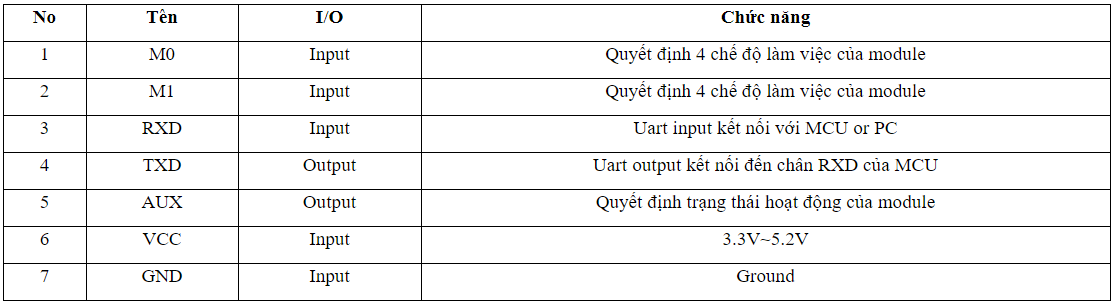
\includegraphics[scale=.5]{Chapter 2/image chapter 2/sodochanvachucnangE32.png}
	\caption[Sơ đồ chân và chức năng của module LoRa E32]{Sơ đồ chân và chức năng của module LoRa E32}
	\label{hinh23}
\end{figure}
\begin{figure}[H]
	\centering
	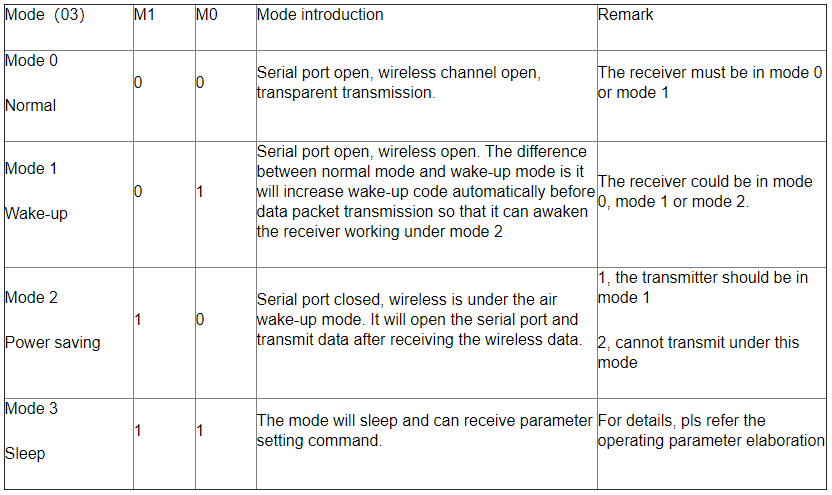
\includegraphics[scale=.5]{Chapter 2/image chapter 2/workmodeE32.png}
	\caption[Chế độ làm việc của module LoRa E32]{Chế độ làm việc của module LoRa E32}
	\label{hinh24}
\end{figure}


\subsection{GIAO THỨC MQTT}
\subsubsection{Khái niệm}
\subsubsection{Nguyên lý hoạt động}
